% Appendix Template

\chapter{Initial Findings Using the Approximation} % Main appendix title

\label{AppendixDef} % Change X to a consecutive letter; for referencing this appendix elsewhere, use \ref{AppendixX}

\lhead{\chaptername~\thechapter. \emph{Initial Findings}} % Change X to a consecutive letter; this is for the header on each page - perhaps a shortened title

%----------------------------------------------------------------------------------------
%    Preamble
%----------------------------------------------------------------------------------------

\section{Preamble}
\label{sec:def_preamble}
This appendix is a paper that was accepted and presented for publication by the International Conference on Lightning Protection (ICLP) in 2014, hosted in Shanghai, China. The paper is entitled: \textbf{\textit{Developing an Approximation to the Heidler Function - With an Analytical Transformation into the Frequency Domain}}.

%----------------------------------------------------------------------------------------
%    Paper Description
%----------------------------------------------------------------------------------------

\section{Paper Description}
\label{sec:def_paper_description}
This paper discusses the preliminary development of the approximation to the Heidler function. It also shows the preliminary results obtained from simulations of the approximation. These results are without any optimisation.

These preliminary results indicated that this approximation is very promising and allowed for further research to optimise the function. The frequency results obtained broadened the scope of the approximation that was developed.

\makeatletter
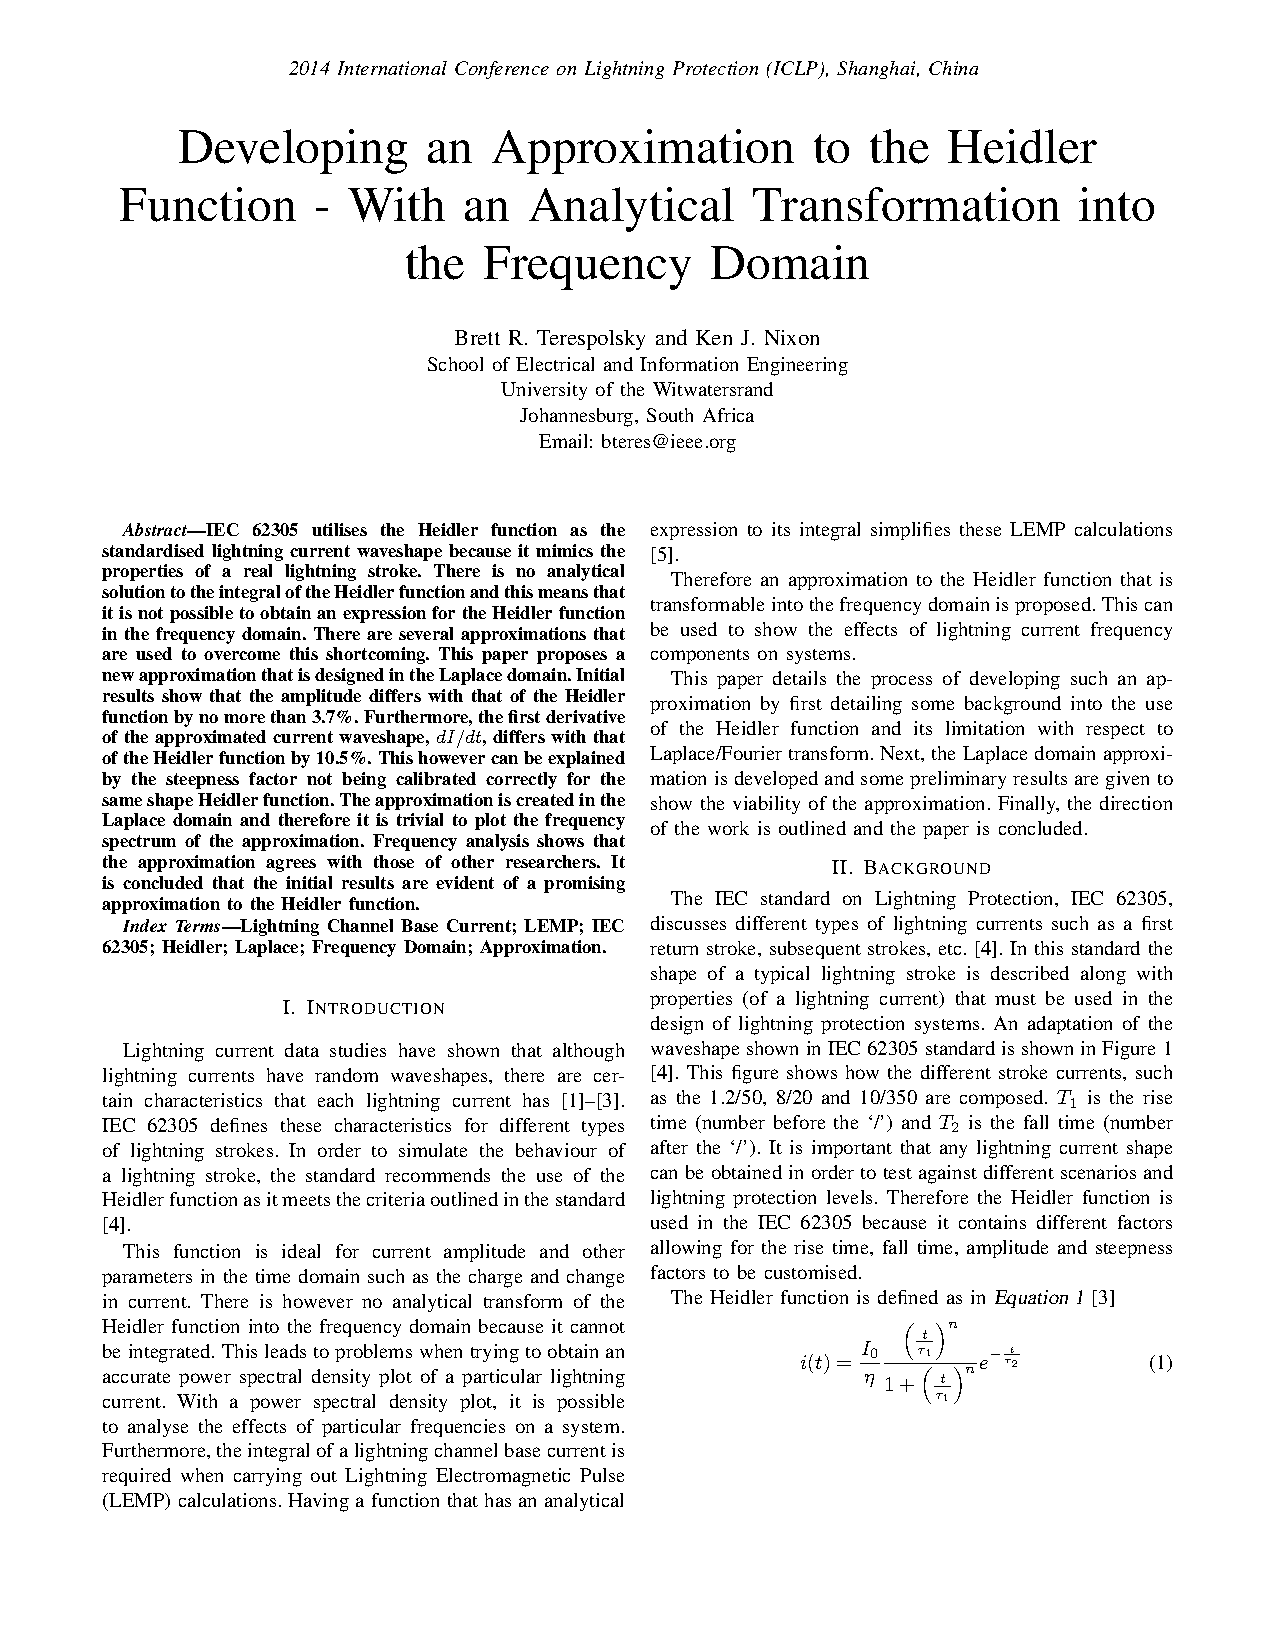
\includepdf[
  pages=-,
  width=\Gm@layoutwidth,
  height=\Gm@layoutheight,
  keepaspectratio=true
]{./AdditionalFiles/BrettTerespolskyICLP2014}
\makeatother
